\documentclass[pdflatex,iicol,sn-basic,Numbered]{sn-jnl}
\usepackage[T1]{fontenc}
\usepackage{lmodern,amsmath,amssymb,booktabs,graphicx,xurl,microtype}
\usepackage[english]{babel}
\raggedbottom
\begin{document}
\hypersetup{pdftitle={Quantum state sonification through Bloch geometry and mutual-information graphs},pdfauthor={}}
\title{Quantum state sonification through Bloch geometry and mutual-information graphs}
% Insert verified author and affiliation commands here before submission.
\abstract{Sonifying a multiqubit state requires choosing which quantum descriptors organize the sound and establishing what survives that choice. We present a deterministic engine combining local Bloch geometry with a maximum spanning forest of pairwise mutual information. Qubit descriptors control sinusoidal voices; breadth-first and depth-first modes organize them into simultaneous frontiers or sequential events. We evaluate 100 development circuits and 100 prospectively held-out circuits of 15 qubits at depths 0--10, producing 2,200 state snapshots and 4,400 primary audio outputs. Analyses account for depth and repeated observations within circuits. In the held-out cohort, adding mutual-information summaries to depth and local descriptors reduces depth-first duration prediction error by 82.01\%, with root-mean-square error falling from 46.65 to 19.78 milliseconds. Synthetic forest controls explain this result: depth-first duration is invariant to connectivity and weight-placement changes that preserve component weight multisets, whereas breadth-first duration changes. Weak Bloch--audio distance associations replicate; the exploratory mutual-information distance association does not. An explicit continuous family of physical states has identical one- and two-qubit marginals and identical final audio within each mode, while central-cut entropy spans 0--7 bits. These results characterize selected descriptor sensitivity and a precise limit to global-state inference. The instrument provides an auditable auditory component for exploratory audiovisual representation and composition; perceptual, usability, and educational benefits remain unevaluated.}
\keywords{Quantum sonification, Bloch geometry, Mutual information, Auditory display, Multimodal interfaces, Reproducibility}
\maketitle

\section{Introduction}\label{sec:introduction}
Quantum computation is commonly represented through circuits, amplitudes, and probability distributions. Rendering selected aspects of this structure as sound poses a representational problem: which mathematical relations become acoustic relations, and which information is lost? Parameter-mapping sonification connects data variables to synthesis controls such as frequency, amplitude, and spatial position \citep{GrondBerger2011}. A multiqubit state makes this choice consequential. Its full description grows exponentially with qubit count, whereas a compact set of local and pairwise descriptors can be inspected and assigned explicit acoustic roles.

These roles also define a sonic form. Simultaneity, succession, envelopes, and spatial organization determine how contributions combine, so sound design is integral to the representation. Vickers and Hogg situate informational and artistic intentions within a shared space of sonification practice \citep{VickersHogg2006}. Here, the compositional motivation concerns explicit data-conditioned constraints on voices and temporal organization. Their computational consequences can be measured without treating aesthetic quality or a listener's understanding as demonstrated outcomes.

Integrated sonification and visualization offers a context for making these correspondences inspectable \citep{Enge2024}. A Bloch ball and a correlation graph can display the descriptors that also control sound. SingingFunction illustrates a different auditory representation of mathematical structure with interactive exploration and listener evaluation \citep{GrondHermann2012}. Our present contribution concerns the auditory engine and its computational characterization. It establishes what a future or accompanying visual interface may legitimately explain, rather than providing evidence of human recognition, usability, or learning.

Quantum sonification already encompasses several representational goals. Kontogeorgakopoulos and Burgarth sonify simulated controlled quantum dynamics through parameter mappings and electroacoustic composition \citep{Kontogeorgakopoulos2014}. Q1Synth connects an interactive Bloch-sphere instrument with qubit state vectors and measurement outcomes \citep{Miranda2023}. The Variational Quantum Harmonizer relates variational optimization to musical organization; the consulted prepublication chapter describes this framework.\footnote{P.~V. Itabora\'i et al., ``Developing a Framework for Sonifying Variational Quantum Algorithms: Implications for Music Composition,'' prepublication chapter, arXiv:2409.07104 (2024), \url{https://arxiv.org/abs/2409.07104}.} Christie and Trayford's preprint instead maps density-matrix structure and coherence in open-system dynamics.\footnote{R. Christie and J. Trayford, ``The Sound of Decoherence,'' arXiv:2412.17045 (2024), \url{https://arxiv.org/abs/2412.17045}.} Tudoce and colleagues combine collective Husimi representations with bipartite entanglement entropy in many-qubit dynamics \citep{Tudoce2026}. These approaches make a claim of first quantum or first multiqubit sonification inappropriate. Their objectives also differ enough that a comparison of architectures does not establish a performance ranking.

\enlargethispage{3pt}
Our engine separates local voice control from relational scheduling. Single-qubit reduced states supply Bloch radius and direction; pairwise quantum mutual information supplies a weighted graph of total correlations, including classical and quantum contributions \citep{Groisman2005}. A maximum spanning forest selects a subset of these relations to organize events. Breadth-first search (BFS) groups qubits in simultaneous frontiers, while depth-first search (DFS) renders them sequentially. The two modes also differ in voice averaging, event durations, and attack envelopes. Their comparison therefore concerns complete rendering configurations. ``Topology'' below means labeled graph connectivity, not a topological phase of matter or spacetime geometry.

A mapping equation alone does not establish an association in the final acoustic descriptors. Oscillator overlap and event scheduling can alter aggregate features. Circuit depth can influence both quantum descriptors and sound, creating pooled correlations that are absent within depth. Moreover, good descriptor-to-audio prediction is compatible with an irreversible representation. Our central question is therefore operational: \emph{which selected local and relational descriptors have measurable acoustic consequences in this circuit ensemble, and what can the representation not identify?}

Five research questions retain the project's original statistical organization, with definitions corrected for repeated observations:
\begin{enumerate}
\item[\textbf{RQ1.}] After removing depth-specific means, are mean Bloch radius and radius-weighted polar angle associated with RMS and spectral centroid, respectively, within each mode?
\item[\textbf{RQ2.}] How do local geometry, subsystem entropy, pairwise correlations, and acoustic descriptors vary with circuit depth?
\item[\textbf{RQ3.}] At each nonzero depth and mode, is radius-weighted azimuthal circular variance associated with stereo channel correlation?
\item[\textbf{RQ4.}] How do the two complete rendering modes differ for the same state, in duration, RMS, centroid, bandwidth, spectral entropy, and spectral flux?
\item[\textbf{RQ5.}] Does adding mutual-information summaries improve descriptor-to-audio prediction beyond depth and local summaries on unseen circuit seeds?
\end{enumerate}

We answer these questions using a development cohort and a separate, prospectively frozen validation cohort. Complementary distance analyses and synthetic forest controls characterize sensitivity and mechanism. Finally, a constructive identifiability argument supplies physical states with different central-cut entanglement but identical audio. The contribution is this combination of an explicit instrument, independently evaluated acoustic behavior, and a provable representational boundary; it is not a general theorem that sound preserves quantum information.

\section{Methods}\label{sec:methods}
\subsection{Circuit ensemble and experimental units}
The primary study uses 100 development seeds (1000--1099) and 100 validation seeds (3000--3099). Each seed generates one ideal 15-qubit circuit trajectory from $|0\rangle^{\otimes15}$, with snapshots after depths $d=0,\ldots,10$. Each nonzero layer applies randomly selected $\sqrt X$, $\sqrt Y$, or $\sqrt W$ single-qubit gates, excluding consecutive repetitions on each qubit, followed by nearest-neighbor $\operatorname{fSim}(\pi/2,\pi/6)$ gates on a one-dimensional chain. The two matchings alternate: $(0,1),(2,3),\ldots$ and $(1,2),(3,4),\ldots$. A private seeded generator ensures prefix consistency. This is a specified one-dimensional ensemble, not a reconstruction of a two-dimensional quantum processor or a quantum-advantage experiment.

Exact classical statevector simulation produces globally pure states without measurements, shots, or noise. Local mixedness arises by partial trace and is not evidence of environmental decoherence. Each cohort contains 1,100 snapshots and 2,200 primary BFS/DFS outputs. Across the primary study there are 200 independent seeds, 2,200 snapshots, and 4,400 outputs; layers and modes are repeated observations, not additional independent experiments. A previously examined cohort (2000--2099) and other earlier exploratory extensions were not used as the prospective test set or pooled into these totals. A technical pilot (seeds 0--2) is also excluded.

The validation specification was frozen in commit \texttt{e968ba6} before generating seeds 3000--3099. This is a local, auditable freeze, not a public preregistration. The renderer corresponds to reference commit \texttt{bb31388}, tag \texttt{paper-pipeline-v1.0.0}; its full hashes and the protocol are supplied in Online Resource 2. No synthesis rule was changed for validation. All 100 validation runs passed the pipeline's recorded technical validation; no failed seed was replaced or excluded from the analyzed cohort.

\subsection{Quantum descriptors}
For qubit $i$, the reduced state is
\begin{equation}
\rho_i=\tfrac12(\mathbb I+\mathbf b_i\cdot\boldsymbol\sigma),\qquad r_i=\|\mathbf b_i\|\in[0,1].
\end{equation}
Its direction is $(\theta_i,\phi_i)$ when defined. Purity and normalized linear entropy satisfy
\begin{equation}
\operatorname{Tr}\rho_i^2=(1+r_i^2)/2,\qquad L_i=1-r_i^2.
\end{equation}
These quantities are mathematically dependent descriptors, not independent quantum resources. Radius-weighted directional summaries use $w_i=r_i\mathbf1\{r_i>10^{-10}\}$:
\begin{align}
\bar\theta_r&=\frac{\sum_i w_i\theta_i}{\sum_i w_i},\\
V_\phi&=1-\left|\frac{\sum_i w_i e^{\mathrm i\phi_i}}{\sum_i w_i}\right|.
\end{align}
Both summaries are defined as zero when the denominator vanishes. Local von Neumann entropies are reported in bits.

Pairwise quantum mutual information is
\begin{equation}
I_{ij}=S(\rho_i)+S(\rho_j)-S(\rho_{ij}),\quad 0\le I_{ij}\le2.
\end{equation}
All 105 pairs are calculated, retaining graph edges with $I_{ij}>10^{-10}$ bits. Numerical negative residuals within the implementation tolerance are clipped; values below $-10^{-8}$ raise an error. The full matrix is saved separately from the maximum spanning forest. Analysis summaries include the retained total $I_{\rm tot}$ and edge-weight entropy
\begin{equation}
H_E=-\sum_{e:p_e>0}p_e\log_2p_e,\qquad p_e=I_e/I_{\rm tot},
\end{equation}
with $H_E=0$ for an empty graph. $H_E$ describes the distribution of weights; it is not bipartite entanglement entropy.

The central bipartition is $A=\{0,\ldots,6\}$ and $B=\{7,\ldots,14\}$. Because the global state is pure, $S_A=S(\rho_A)$ is entanglement entropy across this cut, with $0\le S_A\le7$ bits. It is measured for analysis but is not a direct synthesis input. Neither $S_A$ nor pairwise MI should be conflated with spectral entropy.

\subsection{Frozen voice mapping and scheduling}\label{sec:mapping}
Figure~\ref{fig:architecture} separates the two descriptor pathways. Each qubit drives a sinusoidal voice with
\begin{align}
f_i&=110\,8^{\theta_i/\pi}\ \mathrm{Hz},\\
a_i&=0.22(0.12+0.88r_i),\qquad m_i=0.30L_i.
\end{align}
Before the envelope and stereo gains, its signal is
\begin{equation}
s_i(t)=a_i[1+m_i\sin(2\pi\,6t)]\sin(2\pi f_it).
\end{equation}
Azimuth determines equal-power gains through $p_i=(\phi_i\bmod2\pi)/(2\pi)$, $g_{Li}=\cos(\pi p_i/2)$, and $g_{Ri}=\sin(\pi p_i/2)$. Thus azimuth changes spatial gains, not carrier phase. For $r_i\le10^{-8}$ the renderer substitutes $\theta_i=\pi/2$, $\phi_i=\pi$: an audible, neutral direction for a physically undefined angle. This renderer threshold differs from the $10^{-10}$ threshold for directional summaries.

\begin{figure*}[t]
\centering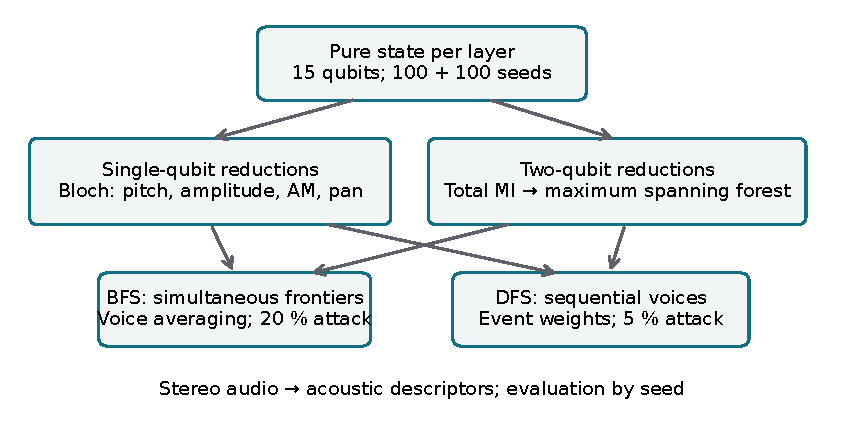
\includegraphics[width=\textwidth]{figures/Fig1_en.pdf}
\caption{Descriptor pathways in the frozen engine. Local reduced states control voices, while the pairwise MI graph selects the forest used for scheduling. Both branches receive the same snapshot. This is an algorithmic schematic, not a screenshot of the audiovisual interface}\label{fig:architecture}
\end{figure*}

Within each forest component, the preferred root is qubit 7 when present and otherwise the smallest label. Components containing the preferred root come first; remaining components are ordered by their smallest label. Neighbors are visited by decreasing edge weight and then label. These choices fix a deterministic, label-dependent traversal; invariance under qubit relabeling is not assumed.

A root lasts 0.30 s; an incoming edge of weight $w$ sets $\tau(w)=0.60-0.25w$ s using the fixed physical range $[0,2]$ bits. Components are separated by 0.12 s. DFS plays each voice separately using its incoming edge and a linear attack/decay envelope with a 5\% attack. BFS plays all voices in a frontier simultaneously, dividing their sum by frontier width, using the mean positive incoming weight for its duration and a 20\% attack. Each event is rounded independently to samples at 22,050 Hz. There is no per-file peak or RMS normalization; frontier averaging is part of BFS. Floating-point WAV files preserve digital amplitude. Combined and continuous listening files are auxiliary and excluded from primary statistics.

\subsection{Acoustic extraction}
A Hann-window short-time Fourier transform (STFT) uses 2,048 samples and 1,536 overlap, with no boundary extension or end padding. Frame power is $P_{kt}=(|X_{L,kt}|^2+|X_{R,kt}|^2)/2$. Centroid and bandwidth are power-weighted frequency mean and standard deviation. Spectral entropy is $-\sum_k u_{kt}\log_2(u_{kt}+10^{-15})$, where $u_{kt}=P_{kt}/\sum_kP_{kt}$; zero-power frames are zero. Flux is the Euclidean distance between consecutive normalized power spectra. Each spectral descriptor is averaged over frames, without discarding silence or weighting frames by energy.

Duration is sample count divided by sample rate. Joint RMS is $\sqrt{\langle(L^2+R^2)/2\rangle}$; stereo correlation is the Pearson correlation between channels, assigned zero if either channel has zero variance. Stereo balance is $(\mathrm{RMS}_R-\mathrm{RMS}_L)/(\mathrm{RMS}_R+\mathrm{RMS}_L+10^{-15})$. All measures are digital signal descriptors. They do not estimate calibrated sound pressure, acoustic energy in joules, perceived loudness, or human discriminability.

\subsection{Statistical specification}
Development results informed the corrected questions and primary endpoint. All subsequent validation models, features, layers, and cohort size were frozen. The independent resampling unit is the complete seed trajectory. Separate test families use Benjamini--Hochberg (BH) false-discovery-rate adjustment \citep{Benjamini1995}; corrected values are denoted $q$. These families do not create a single globally controlled family across the whole paper.

For RQ1, each variable is centered within depth and the pooled Pearson correlation of the residuals is calculated separately by mode. This is one summary of within-depth covariance, not a separate claim of significance at every depth. Whole-seed label permutations (5,000) preserve trajectories; a 5,000-seed bootstrap recomputes centering for confidence intervals (CIs). BH covers four associations. RQ2 reports depth means and pointwise 95\% seed-bootstrap intervals, not simultaneous bands.

RQ3 uses Spearman correlation across 100 seeds separately at each depth 1--10 and mode. Layer 0 is degenerate and excluded. Each of the 20 tests uses 100,000 seed-label permutations, with BH across all 20. RQ4 averages the 11 paired BFS-minus-DFS differences within each seed before a paired $t$ test (99 degrees of freedom). It reports 10,000-seed-bootstrap CIs and BH over six descriptors. Complete layerwise and control tables are included in Online Resource 1.

RQ5 uses separate ordinary least-squares models by mode and target, with duration and flux as targets. $M_0$ contains an intercept and categorical depth; $M_1$ adds $\bar r$, $\bar L$, $\bar\theta_r$, and $V_\phi$; $M_2$ additionally includes $\log(1+I_{\rm tot})$ and $H_E$. Scaling and coefficients use development seeds only. The fitted models are held fixed for a single evaluation on validation seeds, so this is prediction from quantum descriptors to audio, not quantum-state decoding from audio.

The sole primary endpoint is DFS duration improvement,
\begin{equation}
\Delta=\mathrm{MSE}(M_1)-\mathrm{MSE}(M_2).
\end{equation}
For each test seed, squared errors are averaged over 11 depths; 5,000 bootstrap samples of these 100 seed averages provide a 95\% CI. A positive lower bound is the frozen success criterion. The CI is conditional on this fixed training sample and fit, not on retraining the complete procedure. Relative reduction is $100\Delta/\mathrm{MSE}(M_1)$. The other three mode/target combinations are secondary, with pointwise CIs and no joint confirmatory interpretation. Random-generator seeds and settings are recorded in Online Resource 2.

\subsection{Distance associations and forest controls}
The complementary distance analysis uses eight acoustic features: the six RQ4 descriptors plus stereo balance and correlation, standardized separately by mode using development means and population standard deviations. Within each eligible depth, acoustic Euclidean distances are compared with (i) the mean of 15 qubit-aligned Cartesian Bloch distances and (ii) Euclidean distance between the 105 upper-triangular MI entries. The statistic is the unweighted mean of within-depth Spearman distance correlations. The same whole-seed permutation is applied at all depths in each of 5,000 permutations. The 4,950 pairs are dependent; the sample size remains 100 seeds. BH covers four tests, with Benjamini--Yekutieli (BY) adjustment as a dependence sensitivity \citep{Benjamini2001}. Distances with numerical range below $10^{-10}$ are ineligible: Bloch uses depths 1--10 and MI uses 2--10. No distance-bootstrap CI or geometric isometry claim is made. Because duration is one acoustic feature, these tests do not isolate spectral geometry from temporal organization.

Forest controls retain the original Bloch inputs, component node sets, and weight multisets. \emph{Weight shuffle} permutes weights on fixed edges. \emph{Tree shuffle} samples a labeled tree by a uniform Pr\"ufer sequence within each component and permutes weights on its edges, changing connectivity and weight placement together. Node degree and pairwise graph distances are not preserved. Selected depths are 2, 3, 6, and 10; all 100 validation seeds receive 20 replicates per control, rendered in both modes. Including originals gives 32,800 renders and 32,000 control comparisons. Replicates are averaged within state and selected depths within seed before a 5,000-seed bootstrap. The planned observations are BFS duration/frontier count and DFS duration invariance; all other descriptors are exploratory and reported together with pointwise intervals. These synthetic forests test the renderer, not new physically realizable MI matrices or new quantum simulations.

\subsection{Implementation integrity and analytical diagnostics}
The audit checks complete grids, seed disjointness, descriptor consistency across modes, finite values, input hashes, stored prediction reconstruction, and agreement between recorded and independently computed statistics. The closeout package's 1,334 file hashes agree; its five \texttt{src} files are byte-identical to the archived reference. Development audio replay from saved descriptors had passed before this validation. For the new cohort, raw statevectors and WAVs were not part of the compact evidence package: their per-run validation is recorded by the pipeline, while the independent closeout audit verifies supplied matrices, descriptors, tables, and source. The actual validation environment reports Python 3.11.14, NumPy 2.3.5, SciPy 1.17.1, NetworkX 3.6.1, and Qiskit 2.3.0.

Two analytical diagnostics complement ensemble statistics: exact duration identities derived from scheduling, and an external physical-state family proving non-identifiability of cut entropy from final-snapshot audio. They are not additional RQC draws. A coordinate-seam calculation assesses continuity of the frozen azimuth mapping. Their complete derivations and numerical certificates appear in Online Resource 1.

\section{Results}\label{sec:results}
\subsection{Local associations and depth trajectories}
All four RQ1 associations replicate in validation (Table~\ref{tab:rq1}). Radius--RMS correlation is much stronger for DFS than BFS, consistent with separate versus averaged overlapping voices; the table does not constitute an isolated causal comparison of traversal algorithms. Weighted polar angle is strongly associated with centroid in both modes, although it is not a centroid formula.
\begin{table*}[t]
\caption{Validation RQ1: Pearson after within-depth centering. Seed-level 95\% CIs and BH over four tests; 5,000 permutations limit test-value resolution.}\label{tab:rq1}
\centering\small
\begin{tabular}{llrrr}
\toprule
Mode & Association & $r$ & 95\% CI & $q$ \\
\midrule
BFS & $\bar r$--RMS & $0.449$ & $[0.389, 0.500]$ & $0.000200$ \\
BFS & $\bar\theta_r$--centroid & $0.745$ & $[0.710, 0.777]$ & $0.000200$ \\
DFS & $\bar r$--RMS & $0.979$ & $[0.972, 0.985]$ & $0.000200$ \\
DFS & $\bar\theta_r$--centroid & $0.753$ & $[0.717, 0.784]$ & $0.000200$ \\
\bottomrule
\end{tabular}
\end{table*}


Figure~\ref{fig:depth} shows three descriptive trajectories. Mean cut entropy rises in alternating steps to 6.7366 bits at depths 9 and 10. Layers without an interaction crossing the central cut act as $U_A\otimes U_B$ and cannot change its entropy; this explains the paired plateaus. The steps reflect the gate schedule and snapshot sampling, not quantized entropy. Cross-cut gates need not always increase entanglement.

For dimensions $128\times256$, Page's Haar-random pure-state average is 6.63935 bits \citep{Page1993}, below the strict maximum of 7 bits. It is an ensemble mean, not a ceiling for an individual state or for this structured circuit ensemble. The observed late-depth value above that mean does not by itself demonstrate Haar sampling, thermalization, or new many-body physics. Mean Bloch radius falls from 1 to 0.00824, while DFS spectral entropy remains approximately 1.38 after its early change. Quantum cut entropy and acoustic spectral entropy therefore have distinct trajectories.

\begin{figure*}[t]
\centering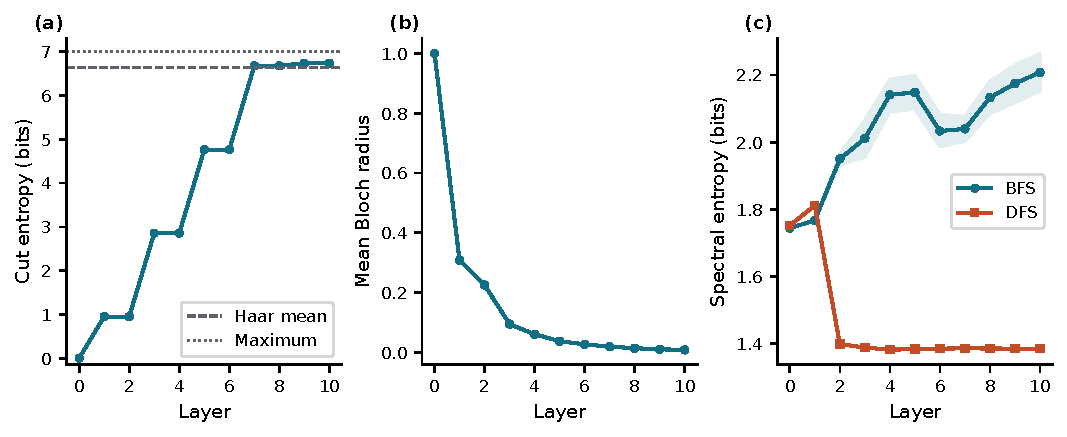
\includegraphics[width=\textwidth]{figures/Fig2_en.pdf}
\caption{Validation depth trajectories: (a) central-cut entropy, with the Haar mean and the maximum distinguished; (b) mean Bloch radius; (c) spectral entropy in each mode. Shading indicates pointwise 95\% seed-bootstrap intervals. Equal cut-entropy values at successive depths follow the alternating interaction schedule}\label{fig:depth}
\end{figure*}

\subsection{Stereo associations and mode contrasts}
RQ3 detects negative associations after BH adjustment at BFS depths 1, 3, and 4 and DFS depths 1, 2, 3, 4, 7, and 10. The early association is not uniform: BFS depth 2 has $\rho=-0.198$ and $q=0.096$, whereas DFS depths 7 and 10 show weaker later associations ($\rho=-0.244,-0.262$; $q=0.033,0.021$). The development cohort had significant negative associations at depths 1--4 in both modes. Thus the broad early relationship is supported, but its complete layerwise significance pattern does not replicate. Circular variance describes azimuthal dispersion; this result is not a test of graph connectivity preservation in stereo.

The paired mode contrasts are shown in Table~\ref{tab:rq4}. BFS is approximately 3.30 s shorter, lower in RMS, and broader in bandwidth, with higher spectral entropy. Its average centroid is only 2.43 Hz higher, despite substantially larger statewise variation. Flux changes from a development null contrast to a small validation difference ($q=0.0465$). This secondary result is reported rather than suppressed; it does not establish that the cohorts differ statistically or that all mode contrasts have equal practical relevance.
\begin{table*}[t]
\caption{RQ4: validation BFS-minus-DFS differences, averaged over all 11 layers within each seed. 95\% CIs and BH over six contrasts.}\label{tab:rq4}
\centering\small
\begin{tabular}{lrrr}
\toprule
Descriptor & Mean difference & 95\% CI & $q$ \\
\midrule
Duration (s) & $-3.301$ & $[-3.348, -3.254]$ & $7.22\times10^{-114}$ \\
Digital RMS & $-0.002410$ & $[-0.002460, -0.002359]$ & $1.47\times10^{-97}$ \\
Centroid (Hz) & $2.426$ & $[1.160, 3.710]$ & $3.82\times10^{-4}$ \\
Bandwidth (Hz) & $51.640$ & $[50.102, 53.187]$ & $3.90\times10^{-82}$ \\
Spectral entropy (bits) & $0.573$ & $[0.560, 0.586]$ & $3.48\times10^{-94}$ \\
Spectral flux & $0.000789$ & $[0.000050, 0.001568]$ & $0.0465$ \\
\bottomrule
\end{tabular}
\end{table*}


\subsection{Held-out prediction: primary endpoint}
The primary DFS duration result satisfies the frozen criterion. $M_1$ and $M_2$ have MSEs 0.00217588 and 0.00039143 s$^2$, respectively. The gain is 0.00178445 s$^2$ (95\% CI [0.00152409, 0.00206287]), corresponding to an 82.01\% MSE reduction and RMSE from 46.65 to 19.78 ms (Fig.~\ref{fig:prediction}). This percentage describes prediction error reduction, not a reduction in the rendered duration or a perceptual improvement.

Depth alone already predicts DFS duration closely: $M_0$ has RMSE 52.31 ms and $R^2=0.998626$. $M_2$ reaches $R^2=0.999803$; the large global $R^2$ should be read beside the absolute error and depth baseline. The incremental result is a replicated encoding consequence, not an independent discovery of hidden quantum information.
\begin{table*}[t]
\caption{RQ5: independent evaluation with fixed training. Positive MSE reduction favors $M_2$. Only DFS duration is primary. Duration MSE is in s$^2$; flux MSE is in squared digital units.}\label{tab:rq5}
\centering\small
\begin{tabular}{llrrr}
\toprule
Mode & Target & MSE $M_1$ & MSE $M_2$ & Reduction (\%) \\
\midrule
BFS & Duration & $0.708880$ & $0.709246$ & $-0.05$ \\
BFS & Flux & $2.04\times10^{-4}$ & $2.04\times10^{-4}$ & $-0.03$ \\
DFS & Duration & $0.002176$ & $3.91\times10^{-4}$ & $82.01$ \\
DFS & Flux & $1.71\times10^{-6}$ & $1.68\times10^{-6}$ & $1.85$ \\
\bottomrule
\end{tabular}
\end{table*}


The BFS duration and flux additions do not improve held-out MSE and their CIs cross zero. DFS flux improves by 1.85\%, with a small positive pointwise interval for the MSE gain. This secondary interval does not carry the primary endpoint's confirmatory status. The asymmetry across modes limits any general claim that relational summaries improve every acoustic target.

\begin{figure*}[t]
\centering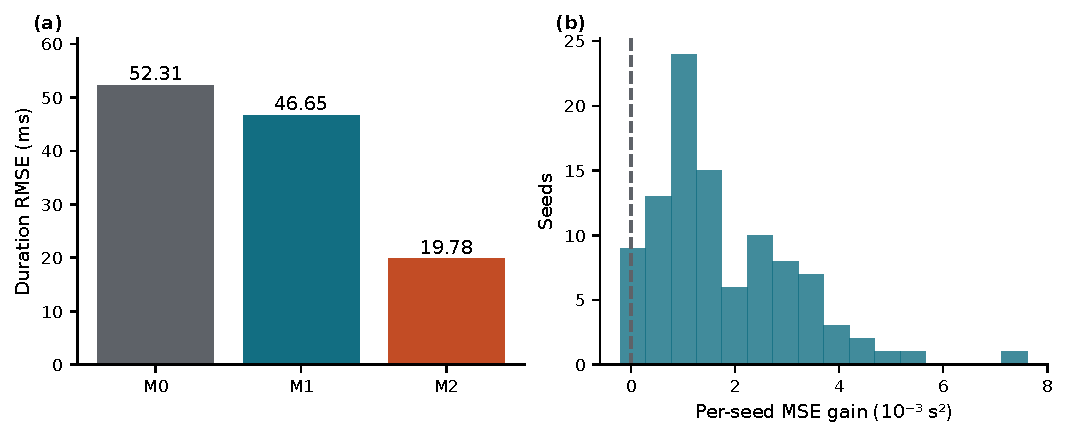
\includegraphics[width=\textwidth]{figures/Fig3_en.pdf}
\caption{Primary validation endpoint. (a) DFS duration RMSE for the depth baseline, local model, and relational extension. (b) Mean squared-error gain per validation seed, averaged across all 11 depths; positive values favor $M_2$. Models and scaling were trained only on development circuits}\label{fig:prediction}
\end{figure*}

\subsection{Mechanistic explanation from forest controls}\label{sec:mechanism}
Let $c$ be the number of forest components and $W$ the sum of forest edge weights in bits. Since a 15-node forest has $15-c$ edges, its ideal DFS duration is
\begin{align}
T_{\rm DFS}&=0.30c+0.60(15-c)\\
&\quad-0.25W+0.12(c-1)\nonumber\\
&=8.88-0.18c-0.25W\quad\mathrm{s}.\nonumber
\end{align}
For BFS, let $F$ count nonroot frontiers across components and let $Q$ sum their mean incoming weights. Then
\begin{equation}
T_{\rm BFS}=0.30c+0.60F-0.25Q+0.12(c-1).
\end{equation}
These identities expose different temporal summaries. DFS duration depends on component count and total retained forest weight, not labeled adjacency. BFS duration also depends on the distribution of nodes and weights among frontiers. Eventwise sample rounding provides the implemented version of these equations.

The independent reconstruction of original DFS sample counts agrees with all 1,100 validation durations within $1.78\times10^{-15}$ s. More importantly, all 16,000 DFS control comparisons have exactly zero duration difference, although tree adjacency changes in all 400 selected states. In contrast, tree shuffle changes BFS duration by $-0.4254$ s (95\% CI [$-0.5207,-0.3383$]) and frontier count by $-0.7905$ ([$-0.9518,-0.6435$]). Weight shuffle leaves frontiers unchanged but changes BFS duration by $+0.01740$ s ([0.01551, 0.01943]); it changes the frontier mean weights. Figure~\ref{fig:controls} summarizes the two manipulations.

These controls support sensitivity to forest organization, while distinguishing a sum invariant from frontier-dependent timing. The tree control does not isolate adjacency from weight placement or degree changes. DFS duration invariance does not imply waveform invariance: reordering and reassigning weights can change spectral and stereo features. Complete exploratory control contrasts remain in the supplement.

\begin{figure*}[t]
\centering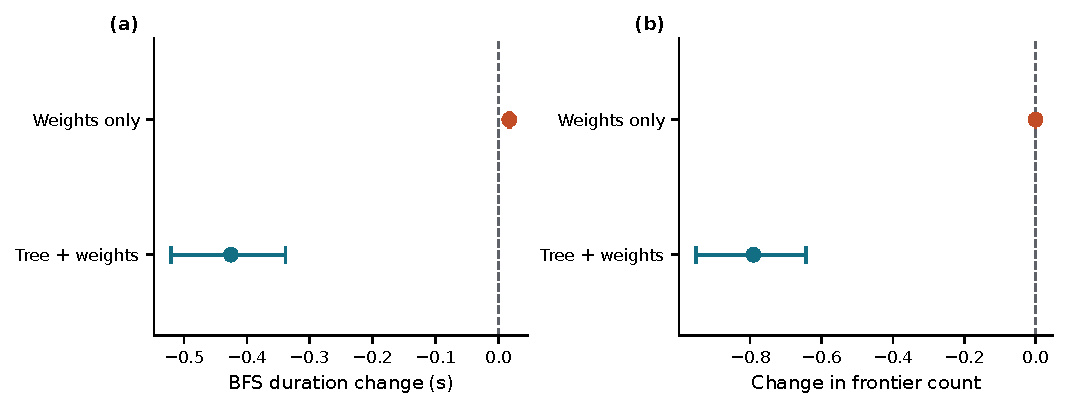
\includegraphics[width=\textwidth]{figures/Fig4_en.pdf}
\caption{Synthetic forest controls in validation. Changes are control minus original, averaged over replicates and selected depths within each seed. Points and bars show means and pointwise 95\% seed-bootstrap intervals. Tree shuffle changes both connectivity and weight placement; weight shuffle retains edges. Both leave DFS duration exactly unchanged}\label{fig:controls}
\end{figure*}

\subsection{Distance associations: partial replication}
The weak positive Bloch--audio distance associations replicate: mean layerwise $\rho=0.0808$ for BFS and 0.1556 for DFS, both BH $q=0.000400$ and BY $q=0.000833$ (Table~\ref{tab:distance}; Fig.~\ref{fig:distance}). Significance does not imply strong geometric agreement or perceptual similarity. No direct test comparing modes' correlation strengths was specified.

MI--audio distance is not supported in the validation family: BFS $\rho=-0.0103$, $q=0.539$; DFS $\rho=0.0330$, $q=0.097$. The exploratory development DFS value was $\rho=0.0536$, $q=0.00213$. Its nonreplication is compatible with the strong DFS duration prediction result: useful low-dimensional weight summaries need not preserve distances between full MI matrices. Nor does a nonsignificant result prove exact independence or a zero population association.
\begin{table*}[t]
\caption{Validation distances: unweighted mean layerwise Spearman, 5,000 whole-seed permutations, and corrections over four tests. Bloch uses layers 1--10; MI uses 2--10.}\label{tab:distance}
\centering\small
\begin{tabular}{llrrrr}
\toprule
Mode & Descriptor & $\bar\rho$ & $p$ & $q_{\rm BH}$ & $q_{\rm BY}$ \\
\midrule
BFS & Bloch & $0.0808$ & $0.000200$ & $0.000400$ & $0.000833$ \\
BFS & MI & $-0.0103$ & $0.539092$ & $0.539092$ & $1.000000$ \\
DFS & Bloch & $0.1556$ & $0.000200$ & $0.000400$ & $0.000833$ \\
DFS & MI & $0.0330$ & $0.072785$ & $0.097047$ & $0.202182$ \\
\bottomrule
\end{tabular}
\end{table*}

\begin{figure*}[t]
\centering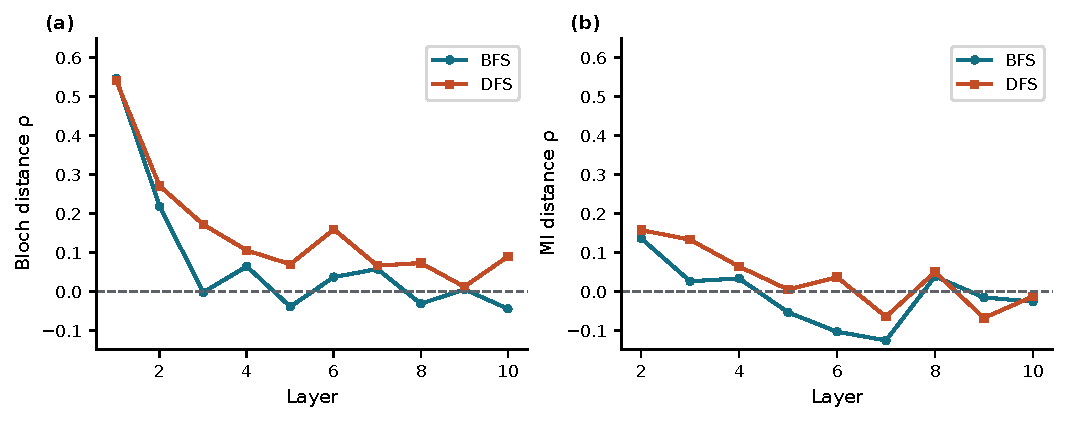
\includegraphics[width=\textwidth]{figures/Fig5_en.pdf}
\caption{Within-depth distance correlations in validation for (a) aligned Cartesian Bloch descriptors and (b) full MI matrices. The overall test averages the displayed correlations and permutes complete seed labels across depths. Degenerate depths are omitted by the fixed numerical rule. The curves have no inferential confidence bands}\label{fig:distance}
\end{figure*}

\subsection{A constructive limit to global inference}\label{sec:nogo}
A compact representation based only on selected reductions can hide genuinely different global entanglement. The general relation between graph-state marginals and multipartite structure is established in quantum-information research \citep{Hein2004,Vandre2025}; the following construction makes the limitation explicit for this engine.

\textbf{Proposition.} Prepare $|+\rangle^{\otimes15}$, apply controlled-$Z$ gates on a seven-node cycle within $A$ and an eight-node cycle within $B$, and apply $\operatorname{CP}(\alpha_i)=\operatorname{diag}(1,1,1,e^{\mathrm i\alpha_i})$ on the seven pairs $(i,7+i)$, $i=0,\ldots,6$. For arbitrary real phases, every one- and two-qubit marginal is maximally mixed, but
\begin{equation}
S_A=\sum_{i=0}^{6}h_2\left(\sin^2\frac{\alpha_i}{4}\right),
\end{equation}
where $h_2$ is binary entropy. At exact descriptor values, $\alpha_i=\pi t$, $0\le t\le1$, gives a continuous family spanning $S_A\in[0,7]$ bits with identical final-snapshot audio within each fixed rendering mode and configuration.

The proof uses cancellation of every one- or two-qubit coherence by an untraced internal cycle neighbor, unaffected by the cross-block matching phase. Internal cycle gates are local to $A|B$ and commute with the matching gates; the cut spectrum is therefore that of seven independent controlled-phase pairs. Online Resource 1 gives the full proof and exhaustive 330-case cancellation certificate. Seventeen numerical states, including heterogeneous phases, corroborate marginal equality and the entropy formula. The archived frozen-engine checks give identical sample arrays within each mode. These are external physical preparations, not draws from the RQC ensemble and not synthetic MI controls. At $S_A=0$, each block remains internally entangled.

Since the final waveform is constant over this family, any estimator using only that waveform has optimal worst-case expected absolute error at least 3.5 bits and mean squared error at least 12.25 bit$^2$ for cut entropy; the constant midpoint estimator attains both bounds. This excludes universal recovery, including learned or randomized estimators, without excluding prediction on a restricted circuit distribution or inference using additional observables, identifying metadata, or preparation history. We present the construction as a characterization of this representation, without claiming priority for the general marginal phenomenon.

\subsection{A coordinate boundary in the frozen panning rule}
The modulo azimuth map has a seam at $\phi=0\equiv2\pi$. Two equatorial pure states with azimuths $\pm\epsilon$ have trace distance $\sin\epsilon\to0$, but their gains approach opposite channels. For the same isolated voice, normalize the stereo-waveform difference by the square root of the sum of the two signal energies. Its squared value is $1-\sin(\epsilon/2)\to1$ (Fig.~\ref{fig:limits}). Thus deterministic rendering does not imply global continuity in physical state distance. A neutral direction at zero radius does not remove this seam at nonzero radius. We retain the frozen mapping and document the limitation; a continuous replacement would define a new instrument version and dataset.

\begin{figure*}[t]
\centering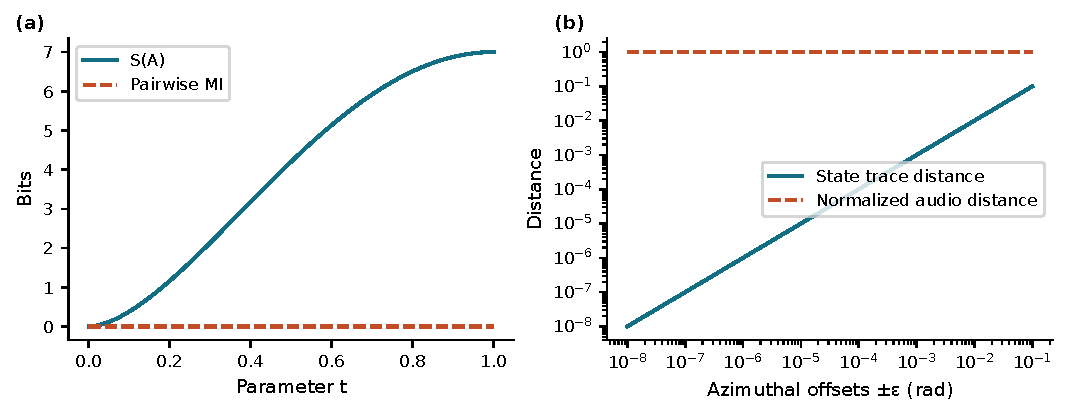
\includegraphics[width=\textwidth]{figures/Fig6_en.pdf}
\caption{Analytical representational limits, separate from the RQC validation cohort. (a) The physical controlled-phase family has variable cut entropy but zero pairwise MI and identical final audio within each mode. (b) Across the azimuth seam, state trace distance tends to zero while normalized isolated-voice audio distance tends to one. Both curves follow exact formulas}\label{fig:limits}
\end{figure*}

\section{Discussion}\label{sec:discussion}
\subsection{What the instrument encodes}
The results support a selective representation. Bloch descriptors have replicated aggregate acoustic associations, and relational summaries substantially reduce a particular prediction error on unseen circuits. The timing identities and controls identify why: DFS compresses forest weight into total duration, whereas BFS also responds to frontier organization. These are useful constraints for designing and explaining an instrument. They do not imply that each audible feature corresponds exclusively to one quantum quantity, or that the final signal permits recovery of the state.

The distinction between the full MI graph and its forest is essential. $M_2$ uses summaries of the full graph, while DFS directly schedules forest weights. The validated prediction is consequently an ensemble relationship between these summaries and the temporal rule, rather than a demonstration that full-matrix geometry is retained. The failed MI distance replication makes that boundary empirically visible. A claim of topology recovery from DFS duration would contradict the exact invariant; a claim of arbitrary cut-entanglement recovery from audio would contradict the physical-state certificate.

The entropy plateaus are also interpretable without introducing speculative physics. They follow invariance under unitaries local to a chosen cut and the alternating schedule of interactions crossing it. Entropy is nonnegative, its maximum is dimensional, and the Page value is a Haar mean. Graphs, entropy, and a resemblance to a staircase provide no evidence here for emergent spacetime, holography, or amplituhedron geometry. Such analogies are outside the demonstrated contribution.

\subsection{Multimodal and compositional implications}
For audiovisual exploration, the most defensible task is to inspect correspondences: select a seed and layer, view local Bloch vectors and the full MI graph alongside its forest, and compare the resulting BFS and DFS outputs. A synchronized interface could highlight active nodes/frontiers and display the exact timing rule. This is a design implication of the verified engine, not an evaluation of an implemented interface in this study. The interface requires separate documentation of its actual controls, synchronization, screenshots, and task flow before it can support interface-specific claims.

The physical-state certificate supplies a particularly useful teaching example: the same local and pairwise display, and the same sound, can accompany distinct entanglement across a larger partition. It demonstrates the difference between a subsystem summary and a global property. Conversely, forest controls illustrate how a fixed set of voices acquires different temporal forms through relational organization. These examples can support an explanation or composition exercise; whether they improve learning or listening remains an empirical question.

Compared with approaches that explicitly sonify bipartite entropy \citep{Tudoce2026}, our cut entropy is an analysis observable rather than a direct timbral parameter. Compared with Q1Synth \citep{Miranda2023}, the emphasis is on multiqubit relational scheduling and repeated-circuit evaluation. These distinctions identify complementary design choices. No shared perceptual or computational benchmark was performed, and no superiority claim follows.

\subsection{Limitations and scope}
Generalization is restricted to an ideal 15-qubit, depth-0--10 circuit ensemble with fixed root, labels, tolerance, and synthesis settings. Seeds are reproducible pseudo-random trajectory identifiers, not random samples of all quantum states. The prospective cohort addresses selection over these circuits; it does not establish robustness to noise, hardware, other gate families, qubit counts, roots, or asymptotic scaling. Exact simulation remains exponentially costly even though output contains only 15 voices. The analytical family establishes a universal failure of injectivity over physical states, while the statistical claims remain distribution-specific.

BFS and DFS vary several synthesis choices simultaneously, so RQ4 cannot attribute differences solely to graph traversal order. The forest is a lossy selection of graph edges, tree shuffle changes multiple graph properties, and distance features include duration. Weak distance associations, pointwise control intervals, and modest or unstable secondary associations should not be presented as a comprehensive preservation result. The panning seam limits continuity and can amplify azimuth differences near its boundary. Digital descriptors do not substitute for hearing tests, and no listener, user, or educational study was conducted.

\section{Conclusion}
A frozen Bloch-and-MI sonification engine can be characterized as a selective quantum descriptor display with reproducible acoustic consequences. Independent circuit validation supports local associations and a strong incremental prediction of DFS duration, while mechanistic controls show that this duration encodes a forest-weight sum rather than full connectivity. Bloch distance associations replicate weakly; MI distance preservation does not receive validation support. A continuous physical-state family proves that central-cut entanglement can vary across its full range while final audio remains unchanged. Together, these results establish what this instrument measures, organizes, and cannot identify. They provide a computational basis for documented audiovisual exploration and composition, with human benefits left to dedicated evaluation.

\backmatter
\section*{Supplementary information}
Online Resource 1 contains additional validation tables, all secondary control contrasts, and proofs of the timing identities, physical-state certificate, and azimuth-seam formula. Online Resource 2 contains analysis data, frozen specifications, source hashes, numerical certificates, and reproduction scripts. The language versions report the same evidence; the Spanish version is supplied for team review.

\section*{Statements and declarations}
\textbf{Data and code availability.} The project repository is \url{https://github.com/valirus/Quantum-Sonification-Bloch-V1}. The accompanying reproducibility package contains development and validation analysis tables, recorded predictions, all compact result tables, the frozen protocol, and the reference renderer source. The full validation evidence archive contains per-seed MI matrices and metadata; full statevector, circuit, and WAV archives are retained in the project runs. A permanent, versioned data-deposit identifier and public availability of all referenced analysis commits must be completed by the authors before submission; the repository URL alone is not represented as a deposit of those archives.

\textbf{Human participants.} The reported experiments use classical simulation and signal analysis and include no human participants or identifiable participant data.

\textbf{AI assistance.} ChatGPT/Codex assisted manuscript drafting, translation, analysis-script preparation, and consistency checks. Numerical conclusions are grounded in the supplied execution records, inspectable datasets, and reproducible calculations. This assistance does not establish authorship; the human authors must verify and approve the final text, analysis, and references.

\textbf{Funding, competing interests, and author contributions.} These author-specific declarations, author names, affiliations, and corresponding-author details must be completed and approved by the author team before submission. No declaration of absent funding or conflicts is inferred here.

\bibliography{references}
\end{document}
